\documentclass[11pt]{article}

\usepackage[margin=0.82in]{geometry}
\usepackage[T1]{fontenc}
\usepackage{lmodern}
\usepackage{microtype}
\usepackage{booktabs}
\usepackage{tabularx}
\usepackage{array}
\usepackage{longtable}
\usepackage{enumitem}
\usepackage{xcolor}
\usepackage{xurl}
\usepackage{hyperref}
\usepackage{fancyhdr}
\usepackage{titlesec}
\usepackage{listings}
\usepackage[most]{tcolorbox}
\usepackage{tikz}
\usepackage{graphicx}
\graphicspath{{figures/}{docs/figures/}}
\usetikzlibrary{arrows.meta,positioning,shapes.geometric}

\definecolor{navy}{HTML}{17324D}
\definecolor{blue}{HTML}{2F5D8A}
\definecolor{lightblue}{HTML}{EDF4FA}
\definecolor{lightgray}{HTML}{F4F6F8}
\definecolor{darkgray}{HTML}{4A5560}
\definecolor{green}{HTML}{2F6F57}
\definecolor{linegray}{HTML}{D8DEE5}

\hypersetup{
  colorlinks=true,
  linkcolor=navy,
  urlcolor=blue,
  citecolor=navy,
  pdftitle={Regional MOM6 and SFINCS for Hurricane Ike},
  pdfauthor={Faezeh Maghsoodifar}
}

\pagestyle{fancy}
\fancyhf{}
\lhead{\small Hurricane Ike: MOM6 and SFINCS}
\rhead{\small Technical Report}
\cfoot{\small \thepage}
\renewcommand{\headrulewidth}{0.3pt}

\titleformat{\section}{\Large\bfseries\color{navy}}{\thesection}{0.7em}{}
\titleformat{\subsection}{\large\bfseries\color{blue}}{\thesubsection}{0.7em}{}
\titlespacing*{\section}{0pt}{1.4em}{0.6em}
\titlespacing*{\subsection}{0pt}{1.1em}{0.45em}

\setlist[itemize]{leftmargin=1.4em,itemsep=0.25em,topsep=0.35em}
\setlist[enumerate]{leftmargin=1.6em,itemsep=0.3em,topsep=0.4em}
\renewcommand{\arraystretch}{1.18}

\lstdefinestyle{terminal}{
  basicstyle=\ttfamily\small,
  backgroundcolor=\color{lightgray},
  frame=single,
  rulecolor=\color{linegray},
  framerule=0.5pt,
  breaklines=true,
  columns=fullflexible,
  keepspaces=true,
  showstringspaces=false,
  xleftmargin=0.5em,
  xrightmargin=0.5em,
  aboveskip=0.7em,
  belowskip=0.7em
}
\lstset{style=terminal}

\newtcolorbox{keybox}[1][]{
  colback=lightblue,
  colframe=blue,
  boxrule=0.7pt,
  arc=2mm,
  left=4mm,right=4mm,top=3mm,bottom=3mm,
  #1
}
\newtcolorbox{evidencebox}[1][]{
  colback=white,
  colframe=green,
  boxrule=0.8pt,
  arc=2mm,
  left=4mm,right=4mm,top=3mm,bottom=3mm,
  #1
}

\newcommand{\code}[1]{\texttt{#1}}
\newcolumntype{Y}{>{\raggedright\arraybackslash}X}
\newcolumntype{L}[1]{>{\raggedright\arraybackslash}p{#1}}

\begin{document}

\begin{titlepage}
\thispagestyle{empty}
\vspace*{1.0cm}
{\color{navy}\rule{\textwidth}{1.2pt}}\\[0.8cm]
{\Huge\bfseries\color{navy} Regional MOM6 and SFINCS for Hurricane Ike}\\[0.35cm]
{\Large Whole-project development, evaluation, and reproducibility report}\\[1.2cm]

\begin{tabular}{@{}ll@{}}
\textbf{Author:} & Faezeh Maghsoodifar \\
\textbf{Platforms:} & NCAR Derecho/Casper and UAHPC \\
\textbf{Framework:} & CrocoDash / regional MOM6 / AutoCF / SFINCS \\
\textbf{Workshop project:} & Regional ocean and coastal flood modeling for Hurricane Ike (2008) \\
\textbf{Report date:} & October 2, 2026 \\
\end{tabular}

\vspace{0.8cm}
\begin{tcolorbox}[colback=white,colframe=linegray,boxrule=0.6pt,arc=2mm,left=4mm,right=4mm,top=3mm,bottom=3mm]
\textbf{Acknowledgments.} This work builds on \textbf{CrocoDash}, the open-source framework for configuring regional MOM6 simulations within CESM \cite{crocodash}. I acknowledge the CrocoDash development team for providing the software foundation used in this work. I would also like to thank \textbf{Dan Amrhein} for suggesting the initial idea that motivated the ERA5 atmospheric-forcing extension, \textbf{Andrew Ross} for his assistance with validation, and \textbf{Manish Venumuddula} for his help with code debugging and software development. Their input and technical support contributed to the development and testing of this extension.
\end{tcolorbox}

\vfill
\begin{keybox}
\textbf{Purpose.} This report documents the Hurricane Ike regional ocean and coastal flood modeling project: regional MOM6 configuration with CrocoDash, development of full ERA5 atmospheric forcing, comparison with CORA, recovery and calendar correction of ocean-boundary products, and construction and evaluation of a Galveston Bay SFINCS baseline with AutoCF. It records completed deliverables alongside the experiment design and remaining MOM6-to-SFINCS integration work.
\end{keybox}
\vfill
{\color{navy}\rule{\textwidth}{1.2pt}}
\end{titlepage}

\tableofcontents
\newpage

\section{Project overview and completed contributions}

The project investigates how regional ocean modeling can supply the offshore water-level signal needed for compound coastal flood simulation in Galveston Bay during Hurricane Ike (2008). The work spans two computing environments: CrocoDash/CESM regional MOM6 preparation and execution on NCAR systems, and AutoCF/SFINCS coastal model construction, GPU execution, and evaluation on UAHPC. The ERA5 extension is one contribution within this wider modeling workflow.

The scientific objective is to distinguish the influence of atmospheric forcing, ocean-grid resolution, and coastal bathymetry on the ocean boundary and subsequent flooding. The available project record includes a completed full-ERA5 MOM6 demonstration and a completed NOAA-boundary SFINCS baseline. Prepared MOM6 boundary files provide the next integration step; a completed nested SFINCS comparison is not established by the saved records.

\begin{table}[htbp]
\centering
\caption{Whole-project deliverables and evidence available in the project archive.}
\begin{tabularx}{\textwidth}{@{}L{0.25\textwidth}Y L{0.24\textwidth}@{}}
\toprule
\textbf{Work component} & \textbf{Deliverable} & \textbf{Recorded status} \\
\midrule
Regional MOM6 & Gulf setup and Hurricane Ike notebooks; GLORYS ocean boundaries and TPXO tides & Baseline marked done in the experiment plan; full-ERA5 run completed \\
ERA5 software & Eight-field preparation, humidity derivation, mesh and stream configuration, deployment bundle & Implemented and demonstrated through 2008-09-20 \\
Ocean evaluation & Pier 21 vicinity comparison with CORA; project figures & Comparison produced \\
Boundary preparation & Texas and Mississippi SSH products, recovery notebooks, checksummed calendar-corrected copies & Files prepared; numerical SSH and time values preserved \\
Coastal modeling & Galveston Bay subgrid SFINCS setup, forcing and terrain provenance, GPU run & AutoCF build and run recorded PASS \\
Coastal evaluation & Two-station water-level scores and maximum-depth map & AutoCF evaluation recorded PASS; extent validation unavailable \\
Experiment framework & E1 resolution, E2 forcing, E3 bathymetry notebooks and comparison plan & Designed/prepared; completion of all sensitivity runs not established \\
\bottomrule
\end{tabularx}
\end{table}

\section{Study domains and regional MOM6 configuration}

Hurricane Ike is the principal demonstration event. The regional parent model covers the Gulf of Mexico at nominal $1/12^{\circ}$ resolution, while the coastal application focuses on Galveston Bay. The MOM6 window is August 30--September 20, 2008; the recorded SFINCS baseline covers September 8--16. The wider Gulf domain represents shelf-scale ocean response before the offshore signal is passed to the finer coastal model.

CrocoDash configures regional MOM6 within CESM using GLORYS ocean initial/boundary information and TPXO tidal constituents. The project notebooks prepare storm-specific cases and sea-surface-height diagnostics for coastal boundary use. The full-ERA5 demonstration retained the ocean-compatible \code{CR\_JRA} coupling contract, with ERA5 replacing the atmospheric data behind that contract.

\subsection{Sensitivity experiment design}

The saved experiment plan defines E0 as the reference, E1 as a finer ocean grid with full-resolution GEBCO, E2 as an ERA5 wind-and-pressure replacement, and E3 as a coastal-bathymetry change relative to E1. The separate full-ERA5 implementation replaces all eight prescribed atmospheric fields and must be distinguished from the original E2 wind-and-pressure-only design.

\begin{table}[htbp]
\centering
\caption{Planned MOM6 comparisons, transcribed from the project experiment design.}
\begin{tabularx}{\textwidth}{@{}L{0.10\textwidth}L{0.15\textwidth}Y L{0.19\textwidth}@{}}
\toprule
\textbf{Run} & \textbf{Grid} & \textbf{Bathymetry and atmosphere} & \textbf{Comparison} \\
\midrule
E0 & $1/12^{\circ}$ & Coarsened GEBCO, minimum depth 5 m; JRA55-do & Reference \\
E1 & $1/24^{\circ}$ & Full GEBCO, minimum depth 5 m; JRA55-do & E0: grid and bathymetry resolution change together \\
E2 & $1/12^{\circ}$ & E0 bathymetry; ERA5 wind and pressure, other fields JRA & E0: atmospheric replacement \\
E3 & $1/24^{\circ}$ & NOAA coastal terrain merged with GEBCO, minimum depth 2 m; JRA55-do & E1: bathymetry and minimum-depth change \\
\bottomrule
\end{tabularx}
\end{table}

Although the plan aims for controlled comparisons, E1 also changes bathymetry resolution and E3 changes minimum depth. Those choices must be harmonized or explicitly reported before attributing differences to a single cause. The prepared notebooks are project deliverables; they are not substitutes for completed run and evaluation records.

\section{ERA5 atmospheric-forcing development}

The extension adds an ERA5 atmospheric-forcing pathway to the original CrocoDash workflow while preserving the existing ocean-compatible CDEPS field contract. The implementation prepares eight atmospheric surface fields from ERA5, derives specific humidity, creates the ESMF mesh required by CDEPS/CMEPS, and connects the prepared variables to the CESM data-atmosphere streams used by regional MOM6.

The tested Hurricane Ike case retained the case configuration name \code{CR\_JRA}. This name reflects reuse of the existing JRA-compatible stream interface; it does not mean JRA data were used. In the tested configuration, all eight prescribed atmospheric fields were supplied by ERA5.

\begin{evidencebox}
\textbf{Runtime evidence from the completed demonstration case}
\begin{itemize}
  \item ERA5 file references in \code{datm.streams.xml}: \textbf{8}
  \item \code{JRA.v1.5} file references in \code{datm.streams.xml}: \textbf{0}
  \item Model execution: \textbf{successful}
  \item Final model date: \textbf{2008-09-20}
\end{itemize}
\end{evidencebox}

\subsection{Software additions to CrocoDash}

\begin{table}[htbp]
\centering
\caption{Main additions implemented for the ERA5 atmospheric-forcing pathway.}
\label{tab:additions}
\begin{tabularx}{\textwidth}{@{}L{0.31\textwidth}Y@{}}
\toprule
\textbf{Addition} & \textbf{Function} \\
\midrule
\code{ERA5AtmosphereConfigurator} & Adds ERA5 as a CrocoDash atmospheric-forcing option. \\
\code{era5\_atmos.py} & Reads and preprocesses ERA5 atmospheric variables. \\
Eight-field conversion & Converts raw ERA5 fields into the atmospheric fields expected by the CESM ocean-coupling workflow. \\
Specific-humidity calculation & Calculates specific humidity from ERA5 dew-point temperature and pressure. \\
Flux/rate conversion & Produces precipitation and radiation rates in forms compatible with the CESM data-atmosphere interface. \\
ESMF mesh creation & Describes the ERA5 0.25$^{\circ}$ grid for CDEPS/CMEPS remapping. \\
CDEPS stream configuration & Connects all eight prepared ERA5 variables to the CESM data atmosphere. \\
Documentation and tests & Documents the workflow and checks preprocessing and stream definitions. \\
Derecho workflow & Retrieves ERA5 from NCAR GDEX and executes the preparation workflow through the tutorial queue. \\
Demonstration case & Runs a successful 21-day Hurricane Ike regional MOM6 simulation using the ERA5 atmospheric streams. \\
\bottomrule
\end{tabularx}
\end{table}

\subsection{Atmosphere--ocean coupling architecture}

The main architectural choice was to keep the existing ocean-oriented CDEPS/JRA field contract and replace the atmospheric datasets behind that interface with ERA5. The implementation therefore does \emph{not} use the land-oriented CESM \code{DATM\%ERA5} pathway.

\begin{figure}[htbp]
\centering
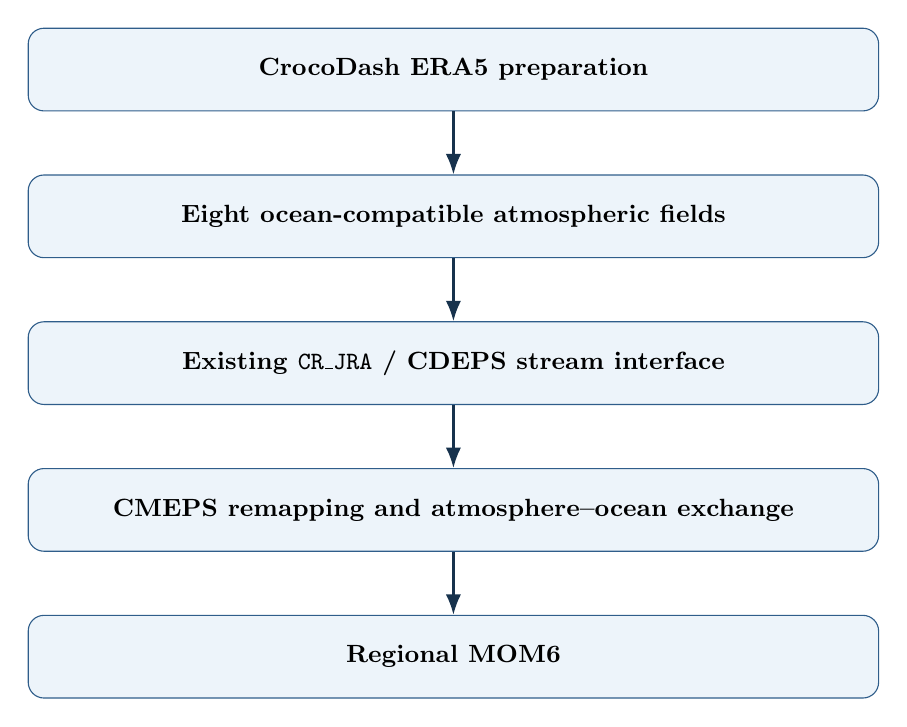
\begin{tikzpicture}[
  node distance=8mm,
  box/.style={rectangle, rounded corners=2mm, draw=blue, fill=lightblue, minimum width=10.8cm, minimum height=1.05cm, align=center, font=\small\bfseries},
  arrow/.style={-{Latex[length=2.6mm]}, thick, draw=navy}
]
\node[box] (a) {CrocoDash ERA5 preparation};
\node[box, below=of a] (b) {Eight ocean-compatible atmospheric fields};
\node[box, below=of b] (c) {Existing \code{CR\_JRA} / CDEPS stream interface};
\node[box, below=of c] (d) {CMEPS remapping and atmosphere--ocean exchange};
\node[box, below=of d] (e) {Regional MOM6};
\draw[arrow] (a) -- (b);
\draw[arrow] (b) -- (c);
\draw[arrow] (c) -- (d);
\draw[arrow] (d) -- (e);
\end{tikzpicture}
\caption{ERA5 atmospheric-forcing architecture used in the tested CrocoDash extension.}
\label{fig:architecture}
\end{figure}

This approach minimizes changes to downstream coupling because the expected CESM/MOM6 atmospheric field names and stream structure remain intact. The new work is concentrated in data access, preprocessing, conversion, mesh generation, and stream construction.

\subsection{ERA5 field preparation}

Table~\ref{tab:fields} summarizes the eight atmospheric fields used in the demonstration. The prepared dataset provides the variables required by the existing atmosphere-to-ocean interface.

\begin{table}[htbp]
\centering
\caption{Mapping from raw ERA5 variables to the prepared CrocoDash/CESM fields.}
\label{tab:fields}
\begin{tabularx}{\textwidth}{@{}L{0.18\textwidth}L{0.18\textwidth}Y@{}}
\toprule
\textbf{Raw ERA5 variable} & \textbf{Prepared field} & \textbf{CESM/MOM6 purpose} \\
\midrule
\code{10u} & \code{u10} & Eastward 10 m wind $\rightarrow$ \code{Sa\_u}. \\
\code{10v} & \code{v10} & Northward 10 m wind $\rightarrow$ \code{Sa\_v}. \\
\code{msl} & \code{msl} & Sea-level pressure $\rightarrow$ \code{Sa\_pslv} and \code{Sa\_pbot}. \\
\code{2t} & \code{t2m} & Near-surface air temperature $\rightarrow$ \code{Sa\_tbot}. \\
\code{2d + pressure} & \code{q2m} & Derived specific humidity $\rightarrow$ \code{Sa\_shum}. \\
\code{mtpr} & \code{precip} & Precipitation rate $\rightarrow$ \code{Faxa\_prec}. \\
\code{msdwswrf} & \code{swdn} & Downward shortwave radiation $\rightarrow$ \code{Faxa\_swdn}. \\
\code{msdwlwrf} & \code{lwdn} & Downward longwave radiation $\rightarrow$ \code{Faxa\_lwdn}. \\
\bottomrule
\end{tabularx}
\end{table}

For this tested case, the atmosphere was therefore fully ERA5 with respect to these eight prescribed surface fields. The retained \code{CR\_JRA} case label indicates interface reuse only.

\subsection{Completed demonstration on Derecho}

The workshop project was tested with a 21-day Hurricane Ike (2008) Gulf of Mexico regional MOM6 case on NCAR Derecho. The prepared atmospheric file and supporting grid files were generated before model execution, and the CDEPS stream configuration was checked to verify that the model referenced ERA5 files rather than JRA files.

The successful completion through September 20, 2008 demonstrates end-to-end execution of the workshop project for the tested period and configuration. The prepared fields, ESMF mesh, CDEPS stream definitions, and model coupling operated together successfully for this case. This case-specific result verifies workflow execution, while broader evaluation across additional domains, dates, and storm conditions would be needed to assess general forcing performance before upstream adoption.


\section{Workshop project workflow and downstream application}

Figure~\ref{fig:workshopflow} summarizes the full project workflow developed during the workshop. ERA5 atmospheric fields are prepared on Derecho and passed through the CrocoDash configuration into the existing CDEPS/CMEPS coupling system for regional MOM6. The MOM6 sea-surface-height output can then provide the ocean-boundary signal for the compound coastal flood modeling workflow, where it is combined with river discharge, rainfall, topobathymetry, roughness, soil infiltration, and atmospheric forcing.

\begin{figure}[htbp]
\centering
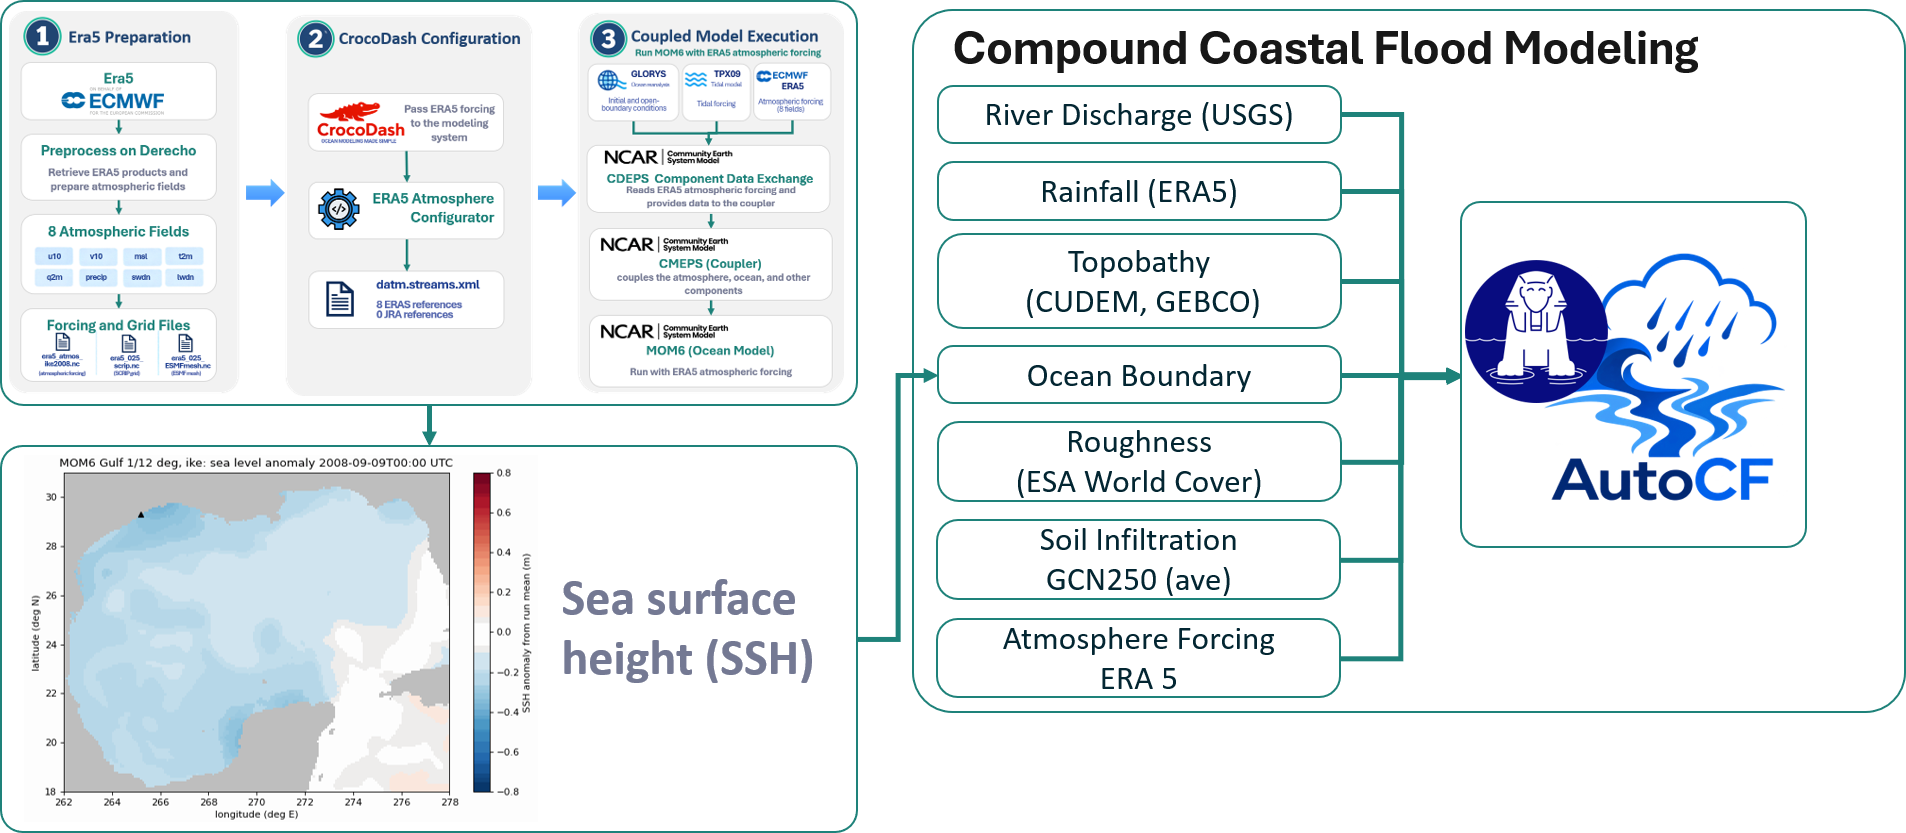
\includegraphics[width=\textwidth]{workshop_project_workflow.png}
\caption{Workshop project workflow linking ERA5 preparation and CrocoDash configuration to ERA5-forced regional MOM6 execution and the downstream compound coastal flood modeling framework. The six stages summarize source data, ERA5 preparation, regional setup, coupling, execution, and output checks.}
\label{fig:workshopflow}
\end{figure}

\clearpage
\section{MOM6 output recovery and boundary preparation}

A dedicated recovery workflow collected sea-surface-height products from the completed \code{gom12\_ike\_ERA5full.001} case for coastal boundary preparation. The archive contains Texas (TX) and Mississippi (MS) regional output files and inventories identifying the original and corrected copies. These products carry sea-surface height in meters and 3,024 records at ten-minute spacing, from August 30, 2008 at 00:10 to September 20 at 00:00. The TX subset has 31 by 55 horizontal points; the MS subset has 29 by 43.

\subsection{Calendar correction and preservation of numerical data}

The source files label their calendar \code{gregorian}, whereas their numeric time axis is interpreted by this project using \code{proleptic\_gregorian}. The handoff documents a two-day displacement when decoding the original metadata. Corrected copies change only the calendar attribute. The corrected manifest explicitly records that neither SSH values nor raw numeric time values were changed and provides SHA-256 checksums for both versions. Recovery and calendar-corrected notebooks preserve the processing sequence.

\subsection{Requirements for an ocean-driven SFINCS boundary}

The remaining boundary workflow must sample MOM6 SSH at the exact SFINCS boundary points, align dates and intervals, and write water levels relative to the coastal model's reference time and vertical datum. Calendar correction alone does not perform this spatial or datum conversion. The project handoff proposes anchoring model anomalies to an observed calm-window mean:
\[
 z_{\mathrm{boundary}}(t)=\eta_{\mathrm{MOM6}}(t)-\overline{\eta}_{\mathrm{MOM6},W}
 +\overline{z}_{\mathrm{NOAA},W}^{\mathrm{NAVD88}}.
\]
Here $W$ is a common pre-storm reference interval. This is a proposed reference-level alignment, not a universal geodetic transformation. The offset and its spatial applicability require checks. The intended variable is SSH (or instantaneous SSH); substituting a differently defined diagnostic without checking its pressure and mean-level conventions would change the boundary signal.

The handoff also requires checking the boundary pressure treatment to avoid double counting an inverse-barometer signal already represented in the parent water level. For the recorded SFINCS configuration, \code{pavbnd = 0} and \code{baro = 1}. A NOAA-versus-MOM6 boundary comparison should use the same built coastal model and forcing, changing only the boundary water-level source.

\section{Galveston Bay SFINCS development and completed baseline}

The coastal component was built with AutoCF and run on UAHPC. The archived \code{galv\_ike2008\_noaa\_sg} configuration uses a 200 m grid in EPSG:32615, with 504 by 564 grid dimensions and a subgrid file. The model window is September 8--16, 2008. The project handoff describes a 10 m subgrid terrain representation, NOAA CUDEM terrain with GEBCO gap filling, land-cover-based roughness, and infiltration inputs.

\subsection{Forcing preparation and boundary quality checks}

The forcing report records NOAA CO-OPS ocean boundaries, AORC precipitation, wind and pressure, and automatically selected USGS discharge. Model preparation included the domain polygon, offshore forcing points, river locations, and observation locations. The handoff identified gaps in automatically selected NOAA boundary records and documented a replacement-boundary procedure using Galveston Pleasure Pier. That quality-control history must be retained when reproducing the final baseline; the provider report alone does not establish the exact final boundary time series.

\subsection{Execution and evaluation record}

The AutoCF command record reports PASS for model build, GPU execution, and evaluation on September 29, 2026. Saved results include maximum water depth, validation-gauge locations, and comparisons at Manchester and Galveston Pier 21. The evaluation scope identifies two scored stations, no independent high-water-mark records, and no remote-sensing flood-extent validation. These results establish a working coastal baseline and its recorded gauge performance, rather than completion of the planned MOM6-driven coastal experiment.

\subsection{Controlled comparison still to complete}

A nested run should reuse the completed coastal model and replace only the ocean boundary with the sampled, calendar-corrected, reference-aligned MOM6 product. Independent interior gauges should be prioritized when scoring the difference, with boundary-forcing gauges identified explicitly. Further experiments can then compare atmospheric, ocean-grid, and bathymetry choices under consistent coastal conditions. Katrina and the earlier Beryl investigation remain contextual or future cases unless separate completed evidence is added.
\section{Project figures and case-specific evaluation}

The figures below complement the runtime checks with the recorded regional MOM6 comparison and downstream SFINCS application. Figure~\ref{fig:mom6cora} evaluates the ERA5-forced MOM6 case against CORA. Figures~\ref{fig:sfincsdomain}--\ref{fig:sfincsvalidation} document a separate SFINCS baseline using NOAA CO-OPS ocean boundaries, AORC atmospheric forcing, and USGS discharge, as recorded in the project forcing report. They are not evidence of a completed ERA5--MOM6-driven SFINCS simulation.

\subsection{Regional MOM6 comparison near Galveston Pier 21}

\begin{figure}[htbp]
\centering
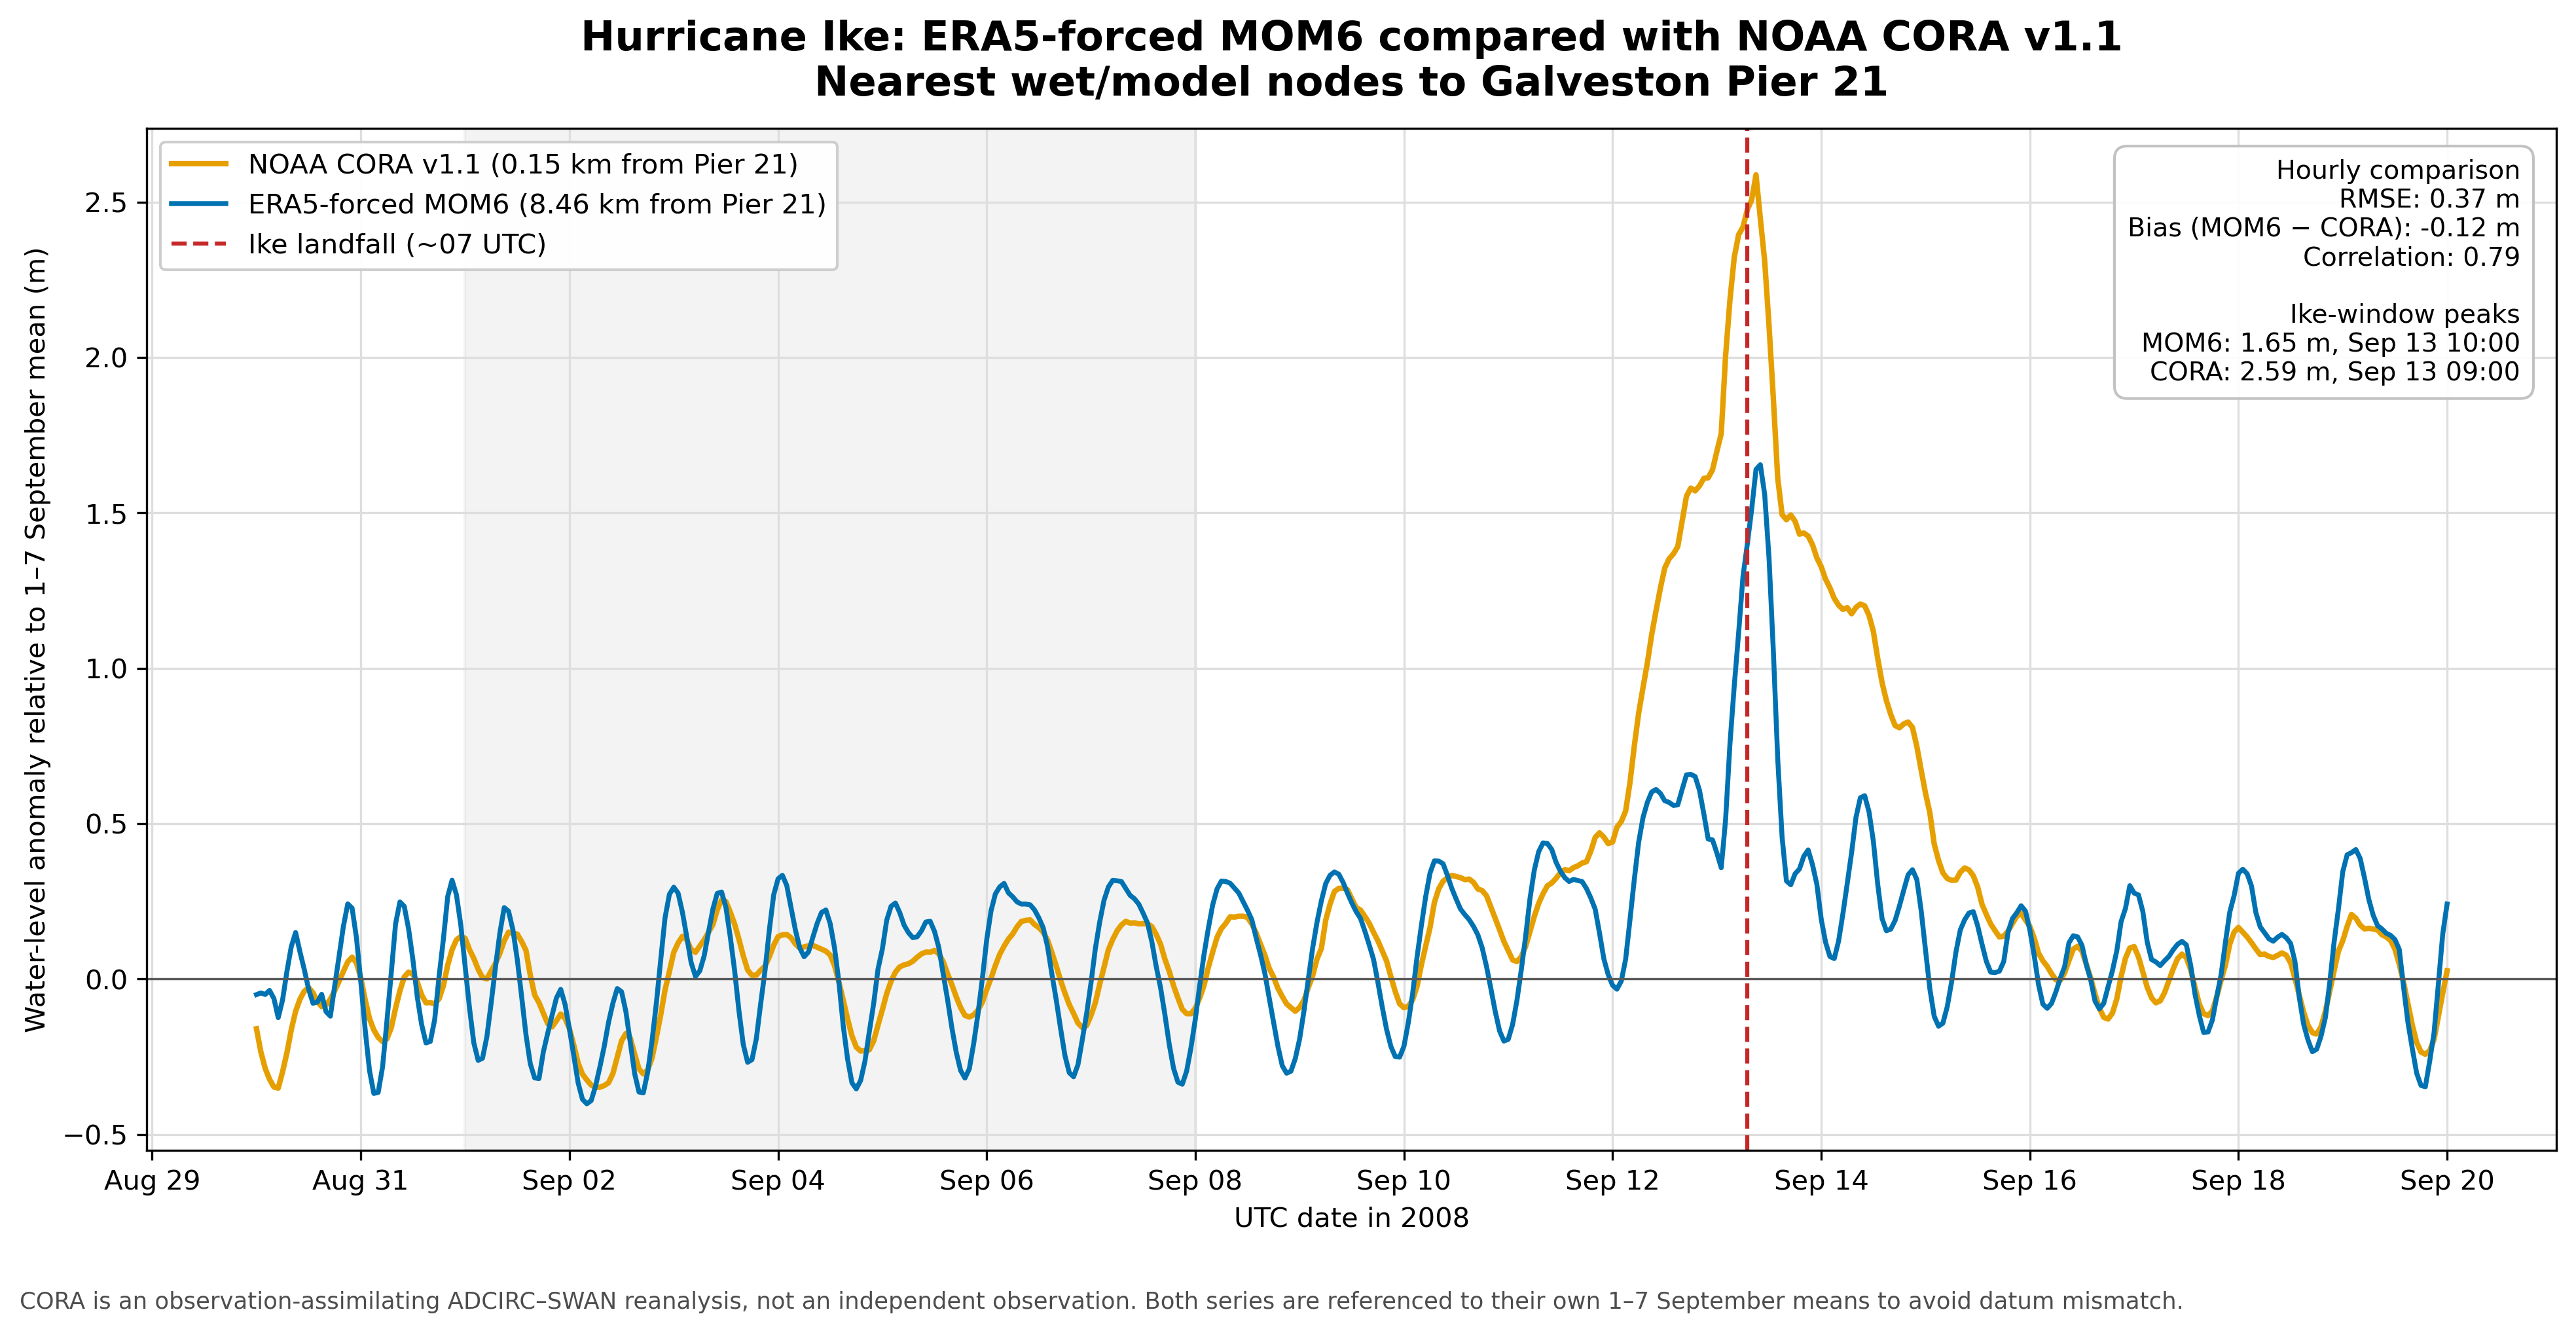
\includegraphics[width=\textwidth]{MOM6_vs_CORA_Ike_Pier21.png}
\caption{ERA5-forced MOM6 and NOAA CORA v1.1 water-level anomalies near Galveston Pier 21 during Hurricane Ike. Each series is referenced to its own September 1--7 mean. The nearest MOM6 wet cell is 8.46 km from Pier 21; the CORA node is 0.15 km away. The plotted hourly comparison gives RMSE 0.37 m, bias (MOM6 minus CORA) $-0.12$ m, and correlation 0.79. CORA is an observation-assimilating ADCIRC--SWAN reanalysis, so this is a model--reanalysis comparison rather than independent gauge validation.}
\label{fig:mom6cora}
\end{figure}

The plotted Ike-window peaks are 1.65 m for MOM6 and 2.59 m for CORA. Spatial sampling, coastal resolution, and differing model formulations must be considered when interpreting this difference; the figure alone does not isolate an atmospheric-forcing effect.

\clearpage
\subsection{SFINCS domain and maximum inundation depth}

\begin{figure}[htbp]
\centering
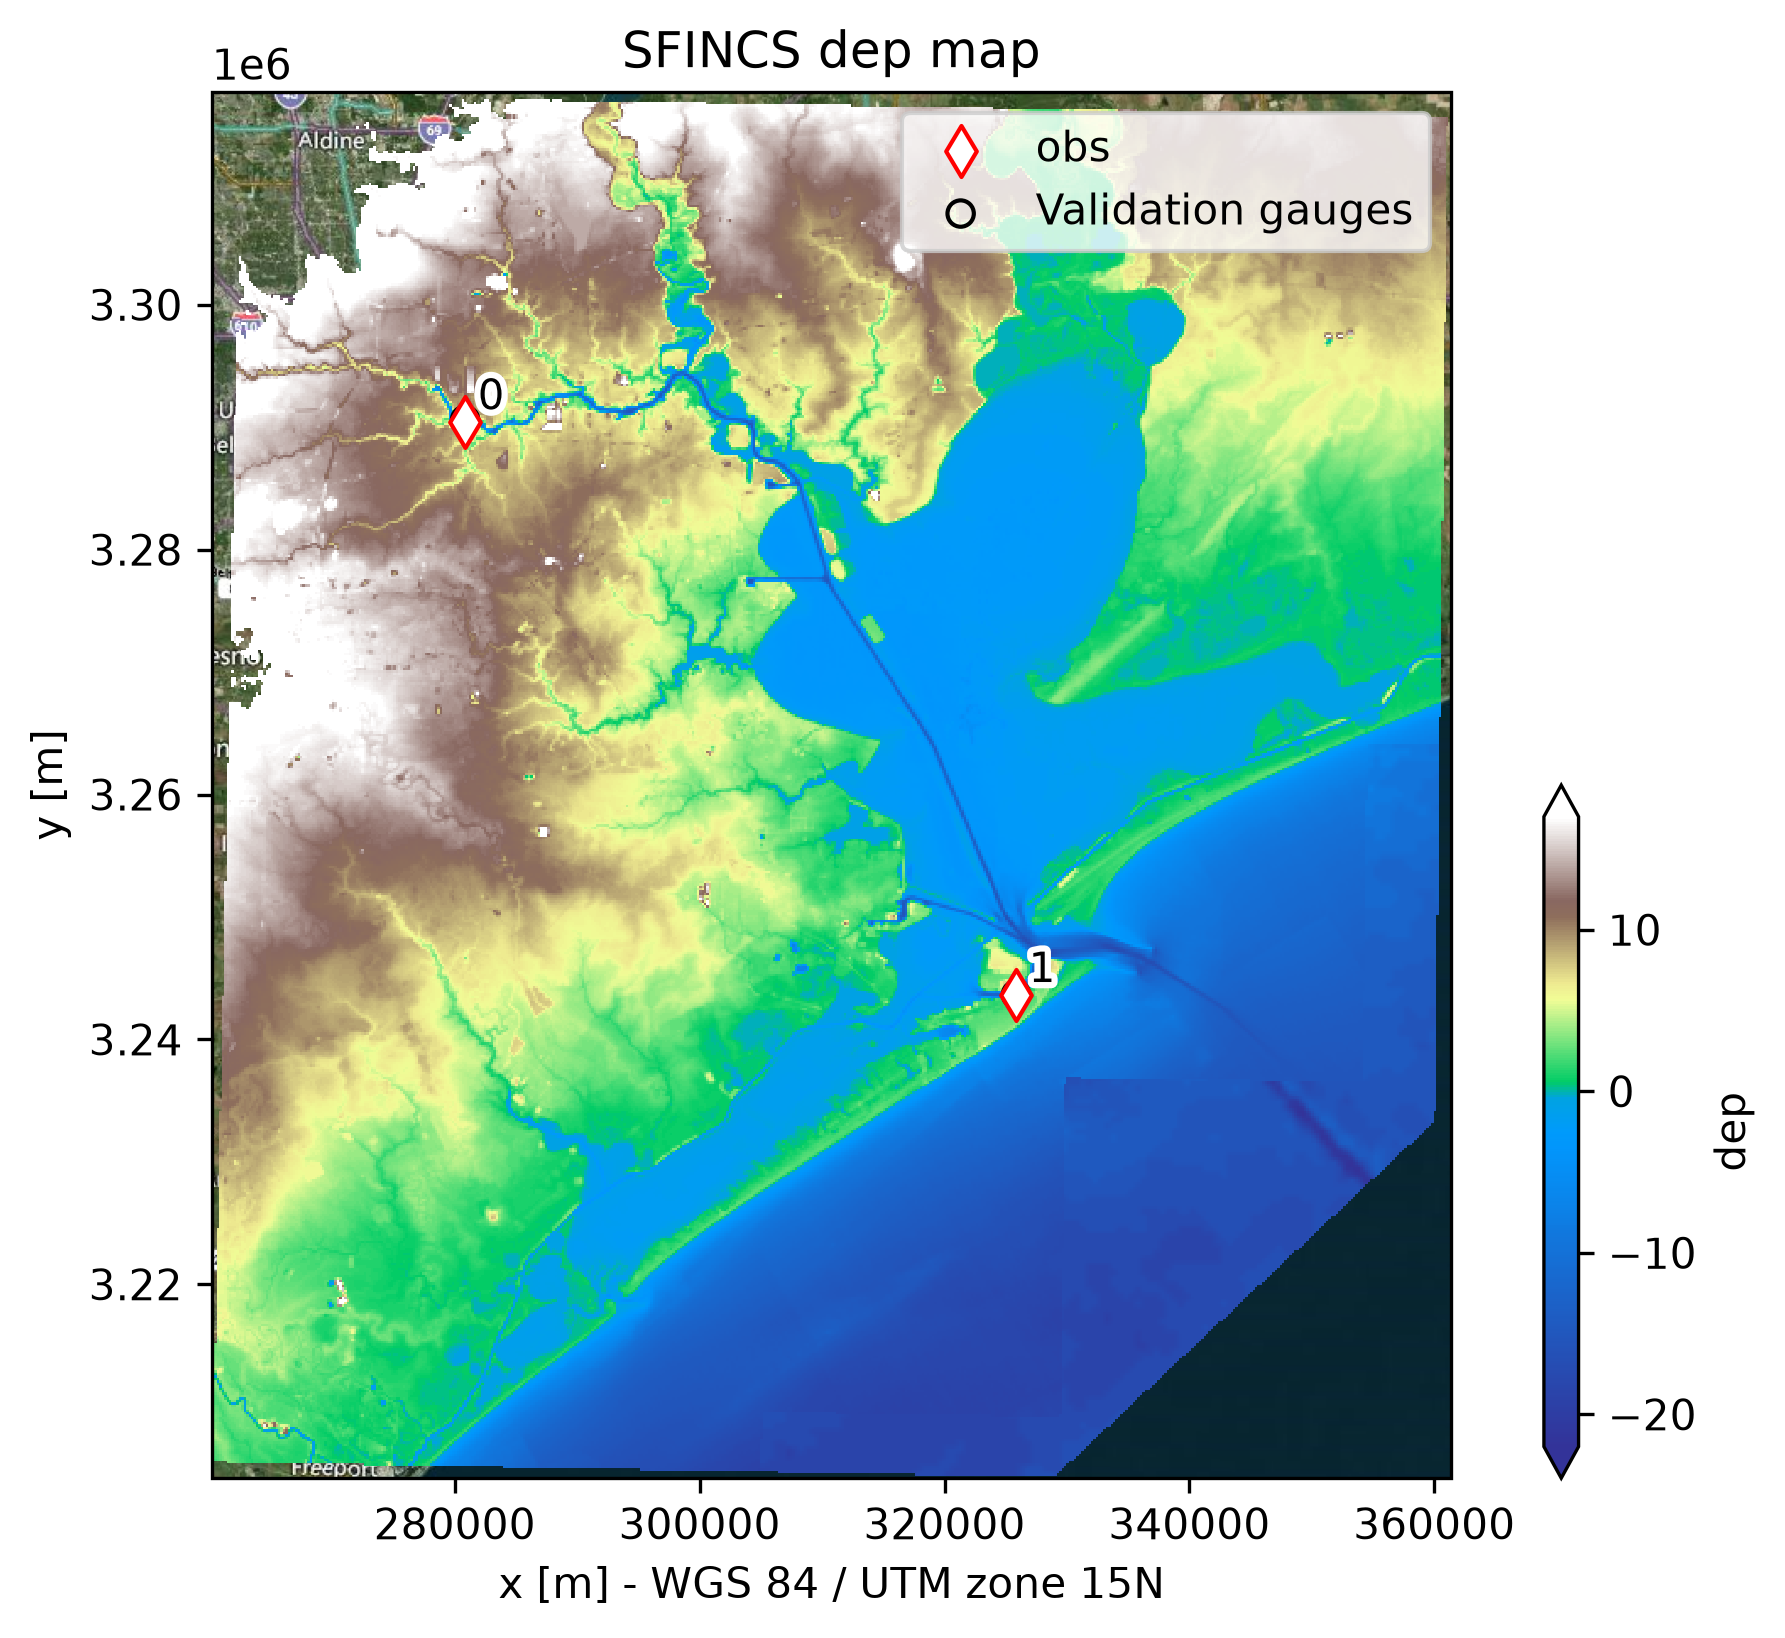
\includegraphics[width=0.78\textwidth,height=0.62\textheight,keepaspectratio]{water_level_gauge_locations_hydromt.png}
\caption{Recorded SFINCS topobathymetry and validation-gauge locations for the Galveston Bay Hurricane Ike application. Coordinates use WGS 84 / UTM zone 15N. The numbered observation markers identify the Manchester and Galveston Pier 21 locations used in the water-level evaluation.}
\label{fig:sfincsdomain}
\end{figure}

\clearpage
\begin{figure}[htbp]
\centering
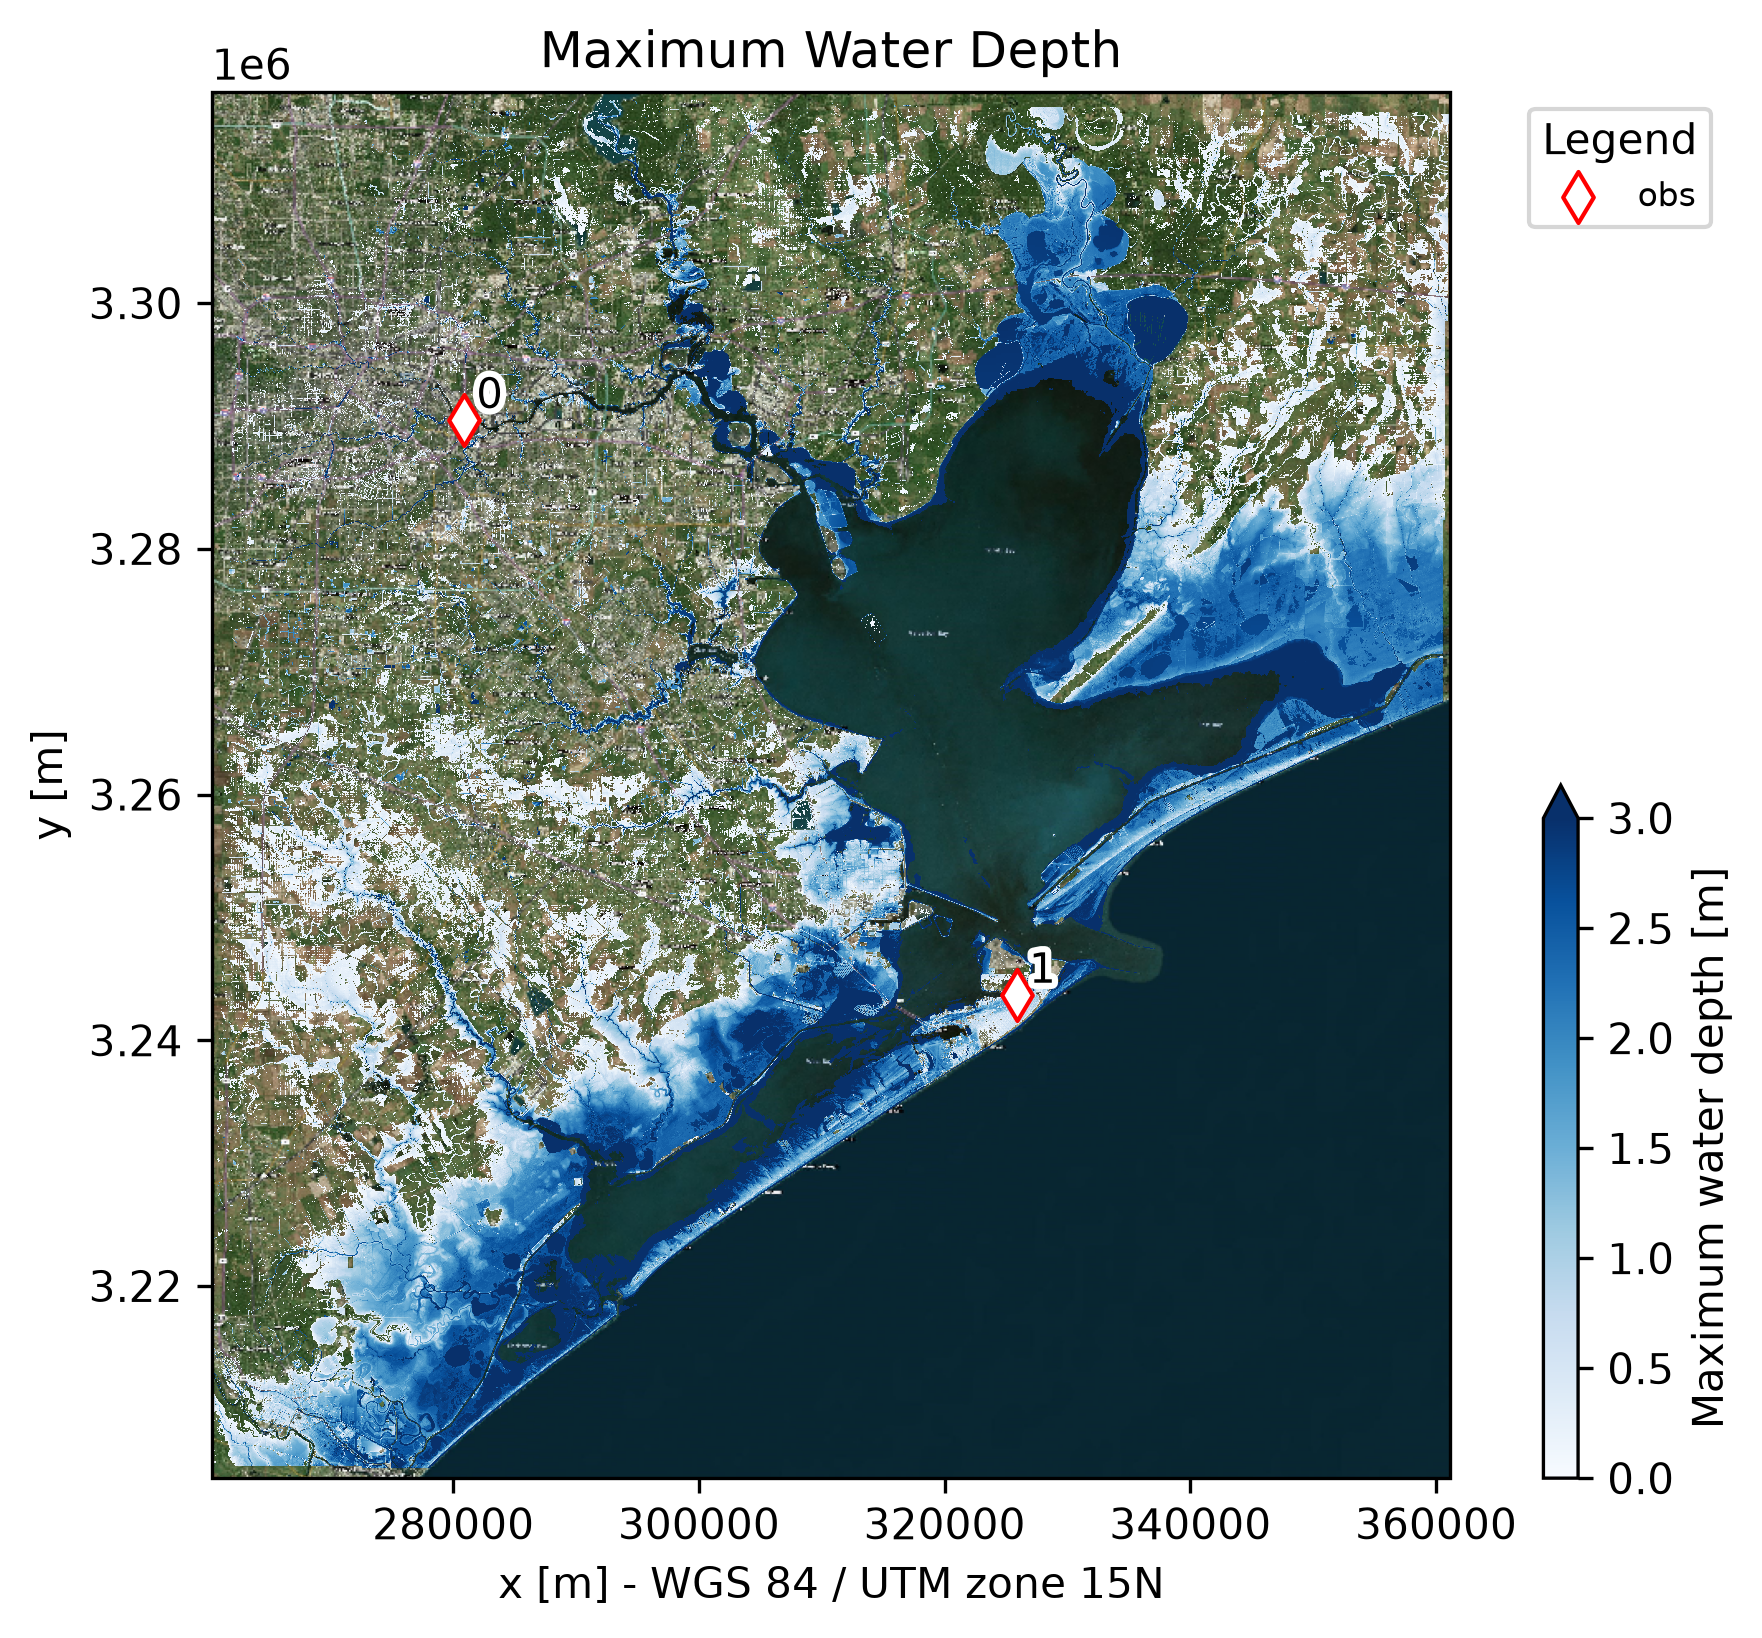
\includegraphics[width=0.78\textwidth,height=0.66\textheight,keepaspectratio]{hmax_subgrid_hydromt_300dpi.png}
\caption{Maximum modeled water depth for the recorded SFINCS baseline, displayed over the Galveston Bay domain with observation-point markers. The color scale is in meters. This model product is not an independently validated flood-extent map; the project evaluation scope records no remote-sensing flood-extent validation or independent high-water-mark assessment.}
\label{fig:sfincsdepth}
\end{figure}

\clearpage
\subsection{SFINCS gauge comparison}

\begin{figure}[htbp]
\centering
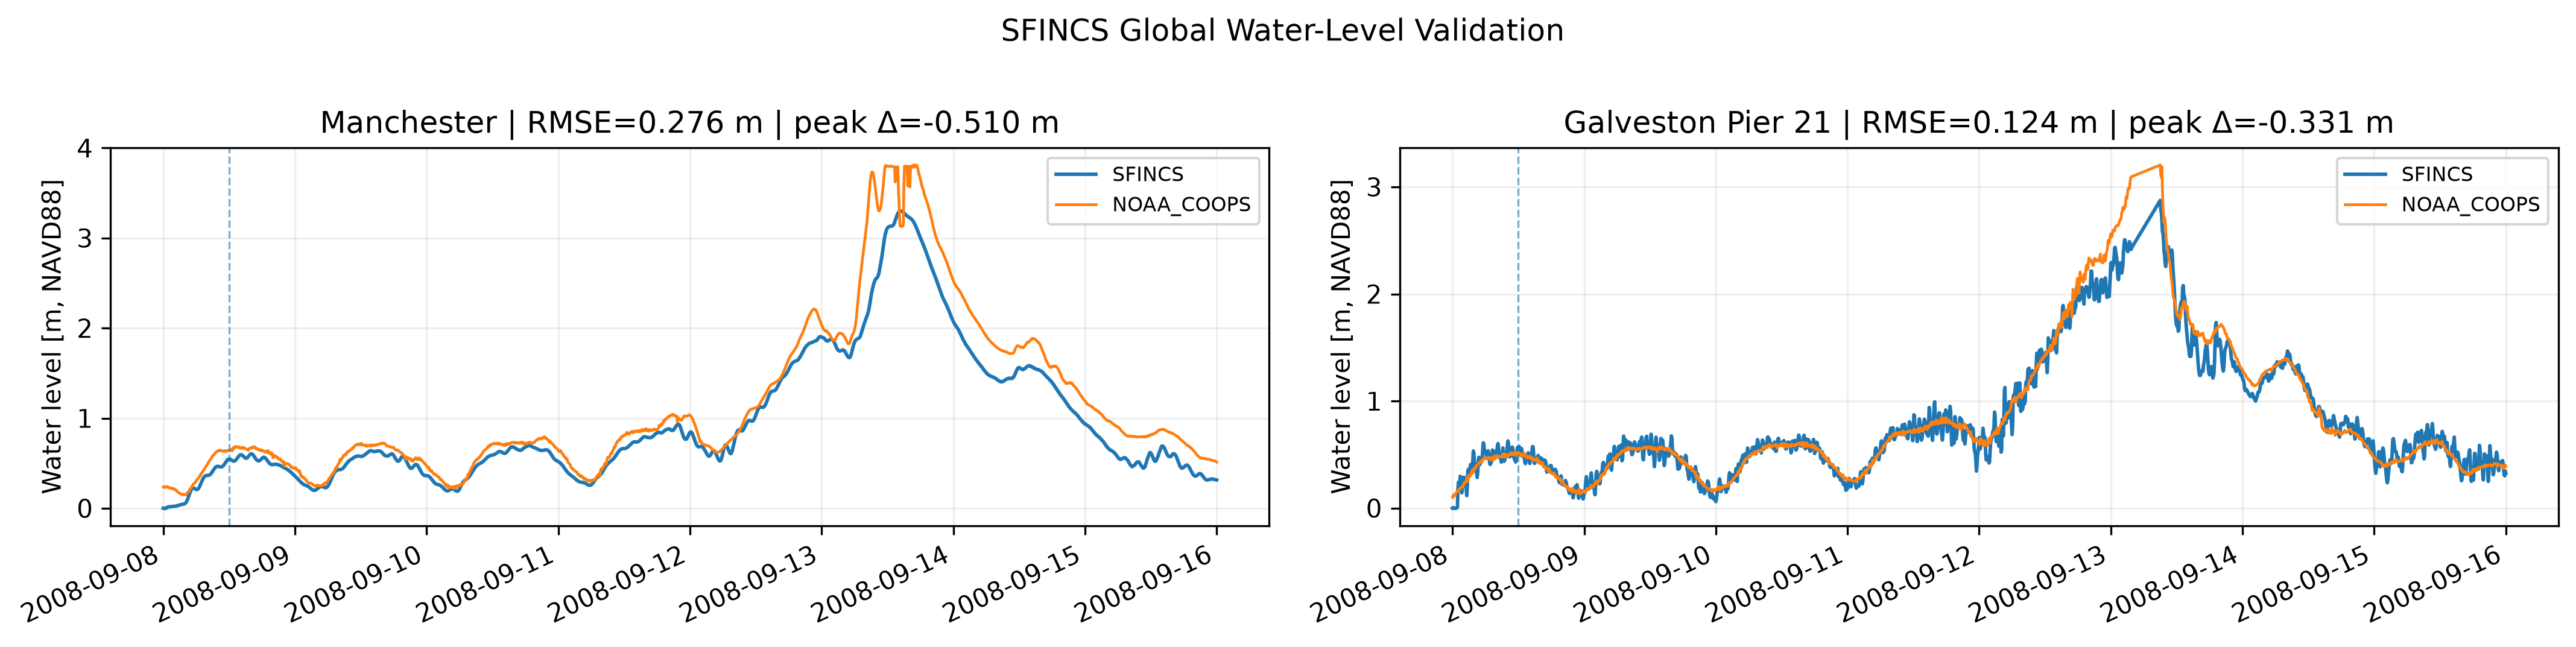
\includegraphics[width=\textwidth]{sfincs_water_level_validation.png}
\caption{Recorded SFINCS baseline water levels compared with NOAA CO-OPS at Manchester and Galveston Pier 21, September 8--16, 2008. Water levels are shown in meters relative to NAVD88. The plotted RMSE values are 0.276 m and 0.124 m, respectively; the reported peak differences are $-0.510$ m and $-0.331$ m. The forcing provenance records NOAA CO-OPS boundary inputs, so these comparisons should be interpreted in that boundary-forcing context.}
\label{fig:sfincsvalidation}
\end{figure}

The gauge comparison documents the available SFINCS baseline evaluation. Repeating the run with prepared MOM6 ocean boundaries and comparing consistent configurations is required to quantify the downstream effect of the ERA5-forced regional ocean simulation.

\clearpage
\section{Reproducibility: inspecting the ERA5 software contribution}

The following commands inspect the local extension and compare it with the current upstream CrocoDash history. They do not rerun the model. The \code{git fetch} command updates remote history metadata but does not alter the working tree.

\begin{lstlisting}
cd /glade/work/faezehmaghso/crocodile2026/CrocoDash-era5

git branch --show-current
git status --short
git log --oneline --decorate -10

git remote get-url upstream 2>/dev/null || \
  git remote add upstream https://github.com/CROCODILE-CESM/CrocoDash.git

git fetch upstream

BASE=$(git merge-base HEAD upstream/main)

git diff --stat "$BASE"..HEAD

git diff "$BASE"..HEAD -- \
  CrocoDash/forcing/atm.py \
  CrocoDash/raw_data_access/datasets/era5_atmos.py \
  tests/forcing/test_era5_streams.py \
  tests/raw_data_access/test_era5_atmos.py \
  docs/source/for_users/3a_configure_forcings.md
\end{lstlisting}

To save the exact contribution as a reviewable patch:

\begin{lstlisting}
git diff "$BASE"..HEAD > \
  /glade/work/faezehmaghso/crocodile2026/era5_crocodash_contribution.patch
\end{lstlisting}

\section{Confirming the prepared forcing files}

The prepared ERA5 directory can be checked with:

\begin{lstlisting}
ERA5DIR=/glade/work/faezehmaghso/crocodile2026/era5_forcing/ike2008

ls -lh "$ERA5DIR"

sha256sum \
  "$ERA5DIR/era5_atmos_ike2008.nc" \
  "$ERA5DIR/era5_025_ESMFmesh.nc" \
  "$ERA5DIR/era5_025_scrip.nc"
\end{lstlisting}

The following lightweight inspection opens the NetCDF metadata and reports only the dimensions, shapes, and units of the eight atmospheric variables rather than loading the full forcing array into memory.

\begin{lstlisting}
/glade/work/faezehmaghso/conda-envs/CrocoDash/bin/python - <<'PY'
import xarray as xr

path = (
    "/glade/work/faezehmaghso/crocodile2026/"
    "era5_forcing/ike2008/era5_atmos_ike2008.nc"
)

ds = xr.open_dataset(path, decode_times=False)

print("File:", path)
print("Dimensions:", dict(ds.sizes))
print("\nAtmospheric variables:")

for name in ["u10", "v10", "msl", "t2m",
             "q2m", "precip", "swdn", "lwdn"]:
    da = ds[name]
    print(
        f"{name:8s} "
        f"dims={da.dims} "
        f"shape={da.shape} "
        f"units={da.attrs.get('units', 'missing')}"
    )

ds.close()
PY
\end{lstlisting}

\section{Collaboration and upstreaming of the ERA5 component}

CrocoDash is a public Python package for setting up regional MOM6 in CESM, and its GitHub repository currently enables issues, discussions, and pull requests. The ERA5 extension falls directly within the package's regional-model setup and forcing workflow. A maintainable upstream contribution should separate the general ERA5 capability from the Hurricane Ike demonstration and remove case-specific assumptions.

Before opening a pull request, the recommended sequence is:

\begin{enumerate}
  \item Open a CrocoDash GitHub Discussion or Issue describing the workshop project, its architecture, and the completed Ike demonstration.
  \item Ask whether maintainers prefer the ERA5 pathway to reuse the existing \code{CR\_JRA} contract or introduce a dedicated atmospheric mode or API.
  \item Generalize the implementation to support arbitrary start/end dates and regional domains, with no hard-coded user names or \code{/glade/work} paths.
  \item Where practical, separate source-specific data access from preprocessing so NCAR GDEX and Copernicus CDS can use the same downstream ERA5 preparation code.
  \item Add automated tests for dew-point-to-specific-humidity conversion, precipitation units, radiation units and sign conventions, latitude orientation, stream calendars/years, and the requirement that the ERA5 pathway produce eight ERA5 stream references and zero JRA data references.
  \item Include a small synthetic or reduced test dataset rather than the multi-gigabyte Hurricane Ike forcing file in the software repository.
  \item Submit code, tests, documentation, and a compact reproducible example as a pull request; keep the full Hurricane Ike reproducibility package in a separate archival record if needed.
\end{enumerate}

\subsection{Suggested collaboration message}

\begin{keybox}
During the 2026 NCAR MOM6/CROCODILE workshop, I developed and tested an ERA5 atmospheric-forcing pathway for regional MOM6 cases created with CrocoDash. The extension prepares eight ERA5 surface fields, derives specific humidity, creates the ESMF mesh, and configures the corresponding CDEPS streams while retaining the ocean-compatible coupling interface.

I tested the workflow on Derecho with a 21-day Hurricane Ike Gulf of Mexico case. The generated \code{datm.streams.xml} contained eight ERA5 stream references and no JRA data references, and the simulation completed successfully.

I would be interested in collaborating to generalize and upstream this capability. I have the implementation, tests, documentation, reproducible notebook, and run evidence available for review. I would appreciate guidance on the preferred CrocoDash API and whether this contribution would be suitable for a pull request and a documented gallery example.
\end{keybox}

\section{Whole-project provenance and reproducibility strategy}

\subsection{Whole-project archive and repository}

The project repository collects notebooks, analysis scripts, experiment and handoff documents, figures, presentations, model configuration, compact evaluation reports, and boundary-file manifests. Large ERA5 forcing, full SFINCS terrain/model outputs, and boundary NetCDF files remain separate from the lightweight repository. The previously uploaded ERA5 bundle is a versioned software dependency; it should be linked and cited rather than presented as the entire ocean--coastal project.

A reproducible whole-project archive should identify both NCAR and UAHPC environments; the exact MOM6 and SFINCS configurations; atmospheric, ocean, terrain, river and gauge data provenance; calendar and reference-level processing; boundary station selection and changes; and checksums for external files. Configuration files retain machine-specific paths and therefore require adaptation in a new environment. The saved source manifest records copied-file provenance; subsequent report revisions belong to the repository history.
\subsection{Source ERA5 data}

Because the demonstration files were obtained from the NCAR GDEX ERA5 collection \code{d633000}, the primary data citation should identify the NCAR-hosted 0.25$^{\circ}$ ERA5 dataset:

\begin{quote}
\textbf{ERA5 Reanalysis (0.25 Degree Latitude-Longitude Grid).} DOI: \href{https://doi.org/10.5065/BH6N-5N20}{10.5065/BH6N-5N20}.
\end{quote}

The corresponding Copernicus ERA5 hourly single-level product can additionally be cited as the originating product:

\begin{quote}
\textbf{ERA5 hourly data on single levels from 1940 to present.} DOI: \href{https://doi.org/10.24381/cds.adbb2d47}{10.24381/cds.adbb2d47}.
\end{quote}

\subsection{Software DOI}

For a standalone software release, a public repository can be connected to Zenodo so that a GitHub release is archived and assigned a DOI. A clean software release should contain the CrocoDash ERA5 source changes, tests, documentation, environment specification, reproducible example notebook, license, and \code{CITATION.cff}; large ERA5 files and credentials should remain outside the software repository.

If the work is merged upstream, DOI and authorship handling should be coordinated with the CrocoDash maintainers so the contribution is represented consistently in upstream release metadata rather than creating a conflicting software record.

\subsection{Processed Hurricane Ike reproducibility package}

A separate archival dataset can preserve the forcing and configuration used for the Hurricane Ike demonstration. A suitable title is:

\begin{quote}
\textbf{ERA5 atmospheric forcing and regional MOM6 configuration for Hurricane Ike (2008), Gulf of Mexico.}
\end{quote}

Potential contents include:
\begin{itemize}
  \item \code{era5\_atmos\_ike2008.nc}
  \item \code{era5\_025\_ESMFmesh.nc}
  \item \code{era5\_025\_scrip.nc}
  \item \code{SHA256SUMS}
  \item \code{README.md}
  \item \code{provenance.yml}
  \item \code{ERA5\_CrocoDash\_NCAR\_setup\_runbook.ipynb}
  \item \code{environment.yml}
  \item selected MOM6 output needed to reproduce key verification results
\end{itemize}

Zenodo currently provides a default 50 GB storage quota per record, so a roughly 7.3 GB forcing package is within the standard per-record limit. The record metadata should identify the NCAR ERA5 DOI as a source dataset using an ``is derived from'' relationship.

\section{Project outcomes and next research steps}

The work produced a regional MOM6 storm workflow, a full-ERA5 forcing extension and completed Ike demonstration, a model--reanalysis comparison, calendar-corrected regional SSH products, and a built, GPU-executed and evaluated Galveston Bay SFINCS baseline. The project also established experiment notebooks, boundary-preparation guidance, provenance records, and a lightweight repository for review and reuse.

The next scientific step is the controlled NOAA-boundary versus MOM6-boundary coastal comparison. This requires completing spatial sampling and reference-level alignment, verifying timing and pressure treatment, rerunning the same coastal configuration, and evaluating at gauges whose role in boundary forcing is explicit. Subsequent sensitivity runs should address confounding changes in grid resolution, bathymetry resolution, and minimum depth before drawing conclusions about the dominant source of improvement.

The final research product should link the whole-project report and repository, the existing ERA5 software release, external data manifests and archives, and the completed experiment records. This structure preserves the distinct achievements of the ocean, software, boundary-processing, and coastal-model components while making the remaining integration work visible.

\section*{References and project links}
\addcontentsline{toc}{section}{References and project links}

\begin{thebibliography}{9}
\bibitem{crocodash}
Venumuddula, M.; Altuntas, A.; Janney, A.; Levy, M.; Milanese, E.; Bailey, D.; Kwong, A.; Hung, N.; and Amrhein, D. (2026). \textit{CrocoDash} (Version 1.0.0) [Computer software]. Zenodo. \href{https://doi.org/10.5281/zenodo.17342301}{https://doi.org/10.5281/zenodo.17342301}. Source code: \url{https://github.com/CROCODILE-CESM/CrocoDash}. Citation metadata from the official \code{CITATION.cff} file.
\end{thebibliography}

\noindent\textbf{Additional project and data links}
\begin{itemize}
  \item CrocoDash citation metadata: \url{https://github.com/CROCODILE-CESM/CrocoDash/blob/main/CITATION.cff}.
  \item CROCODILE-CESM organization: \url{https://github.com/CROCODILE-CESM}.
  \item NCAR GDEX ERA5 dataset d633000 citation record: \url{https://gdex.ucar.edu/datasets/d633000/citation/}.
  \item Copernicus ERA5 hourly single-level product: \url{https://cds.climate.copernicus.eu/datasets/reanalysis-era5-single-levels?tab=documentation}.
  \item GitHub guidance for Zenodo DOIs: \url{https://docs.github.com/en/repositories/archiving-a-github-repository/referencing-and-citing-content}.
  \item Zenodo storage quota guidance: \url{https://help.zenodo.org/docs/deposit/manage-quota/}.
\end{itemize}

\end{document}
